%%%%%%%%%%%%%%%%%%%%%%%%%%%%
% DOCUMENT SETUP & IMPORTS
%%%%%%%%%%%%%%%%%%%%%%%%%%%%
\documentclass[10pt,letterpaper,oneside,english]{article}
\usepackage[margin=.5in]{geometry}
\usepackage[utf8]{inputenc}
\usepackage{setspace}
	\onehalfspace

\usepackage{enumerate}
\usepackage{graphicx}
\usepackage{hyperref}
\usepackage{xcolor}

% \usepackage{enumitem}
% 	\setenumerate[1]{label=\textit{\arabic*}}
% 	\setenumerate[2]{label=\textbf{\alph*},topsep=0pt}

%%%%%%%%%%%%%%%%%%%%%%%%%%%%
% USER-DEFINED COMMANDS
%%%%%%%%%%%%%%%%%%%%%%%%%%%%
% Usage: \person{<last>}{<first>}{<email>}
\newcommand{\person}[3]{
	#1, #2\\
	\href{mailto:#3}{\texttt{#3}}
}
\newcommand{\ncomp}{\emph{non-complete}}


\newcommand{\prog}{\emph{in progress}}

\newcommand{\see}[1]{(see {\color{blue!60!black}\nameref{#1}})}

\newcommand{\chref}[2]{\href{#1}{{\color{blue!60!black}#2}}}

\newcommand{\wref}{\href{http://en.wikipedia.org/wiki/Main_Page}{({\color{blue!60!black}from Wikipedia})}}

\newcommand{\solution}{\newline \hspace*{1em} \textbf{Solution: }}

\newcommand{\code}[1]{\texttt{#1}}

\newcommand{\citem}[1]{\item \code{#1}}

\newcommand{\gls}[2]{ \ \\ \hspace*{1em} \textbf{#1} \ \\ \hspace*{1.5em}{#2}}


%%%%%%%%%%%%%%%%%%%%%%%%%%%%
% TITLE AUTHORS AND DATE
%%%%%%%%%%%%%%%%%%%%%%%%%%%%
\title{
	\textbf{Game Engine Development Team}\\
	Intermediate Report v1.0
}

\author{
	\person{Bahr}{Dan}{dbahr92@gmail.com}
	\and
	\person{Bard}{Etan}{ebard@ups.edu}
	\and
	\person{Burns}{Nick}{nbburns@ups.edu}
	\and
	\person{Livingston}{Chris}{christopherlivingston92@gmail.com}
	\and
	\person{Wilson}{Robin}{rkwilson@ups.edu}
}
\date{\today}



%%%%%%%%%%%%%%%%%%%%%%%%%%%%
% DOCUMENT
%%%%%%%%%%%%%%%%%%%%%%%%%%%%
\begin{document}
\maketitle
\newpage

\tableofcontents
\newpage

\section{Abstract}
The game development group is creating a stand-alone survival/platform game, which will also be capable of taking inputs from a Kinect and mobile phones. Once completed, this project will provide a simple to learn, hard to master style of play, in which players will compete against people using mobile phones.

This document covers the current state of our progress in creating this game. The implementation steps we have taken to create this game, as well as the class-level design behind the scenes, will portray how we have adhered to the deadlines outlined in our timeline. As we are roughly half way into development, this document will additionally provide insight into what challenges we have faced thus far and what we will be focused on for the future.

\section{Design Summary}
\subsection{Class Diagram}
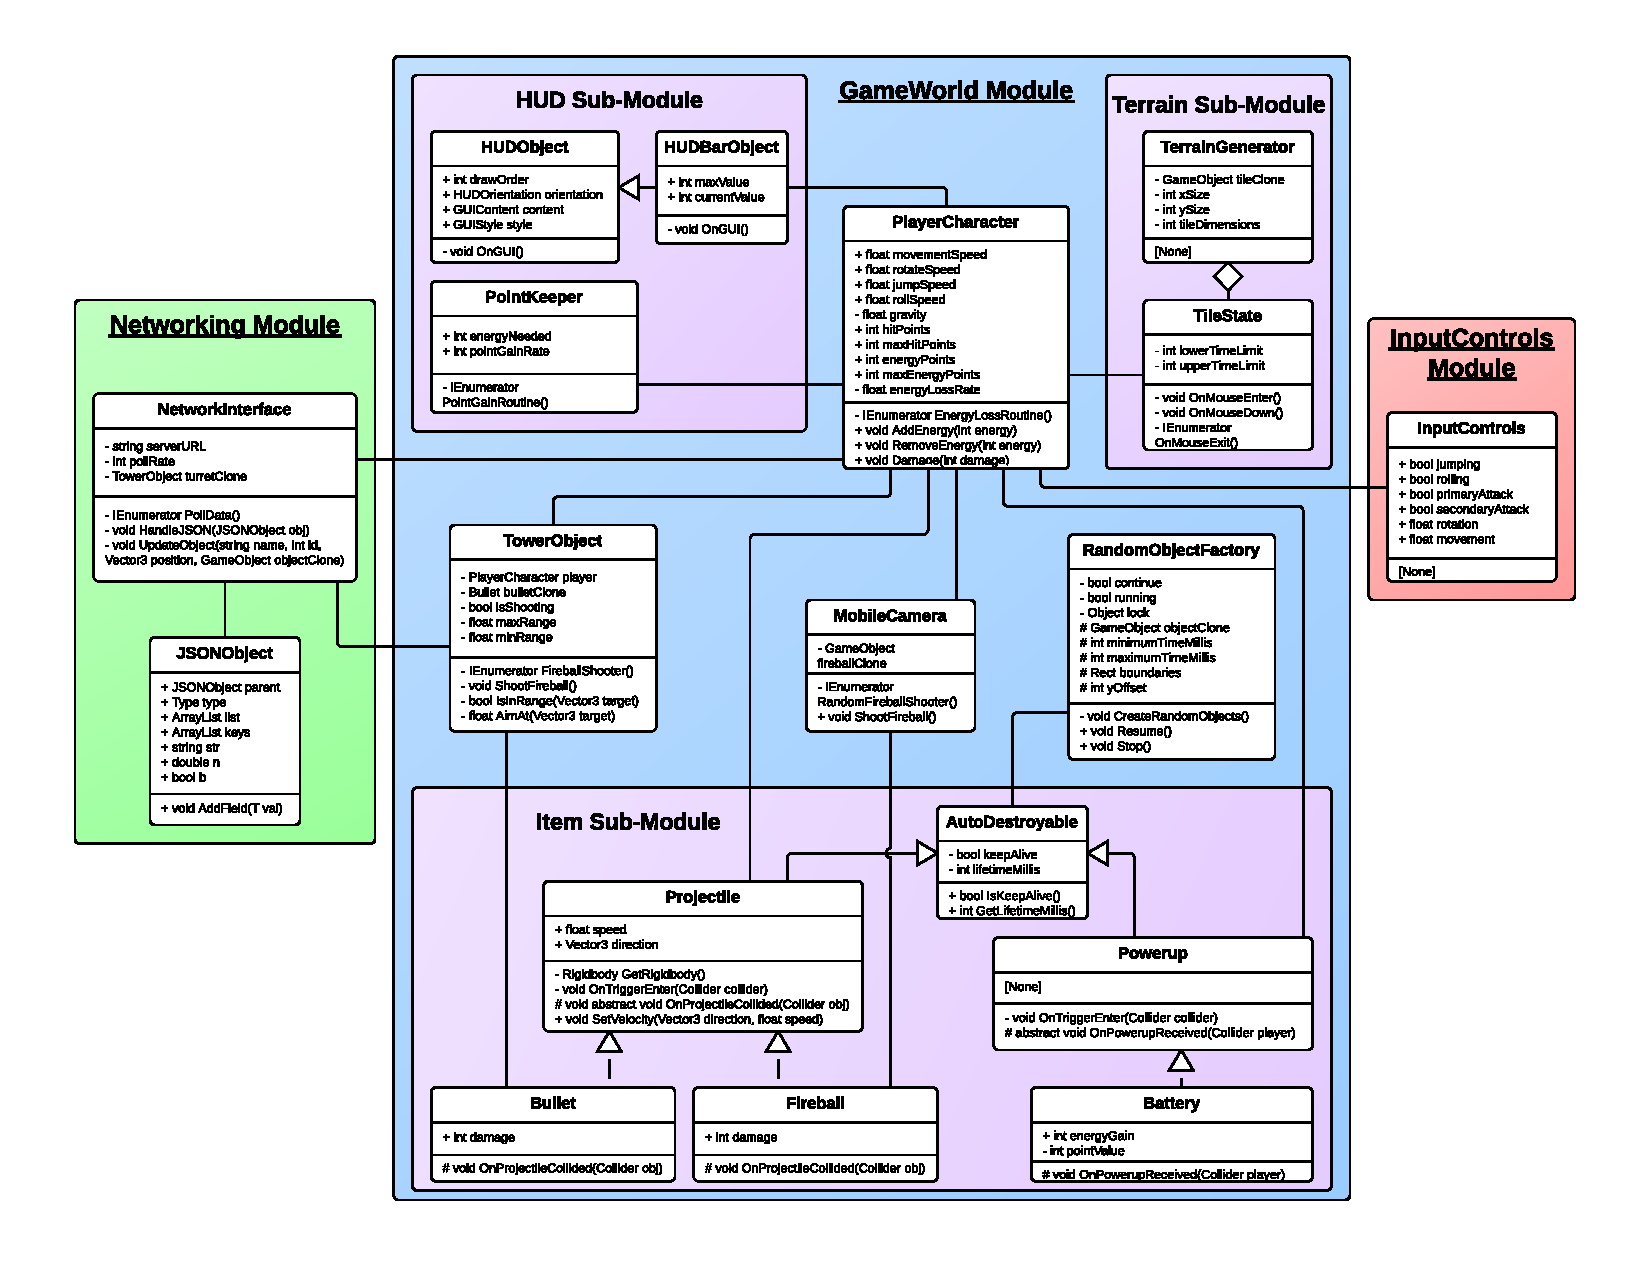
\includegraphics[scale= 0.7]{ViCharClassDiagram}

\subsection{Class Diagram Description}
Three major modules exist: the GameWorld, InputControls, and Networking. The GameWorld includes several classes (PlayerCharacter, MobileCamera, TowerObject, Battery, Projectile, and TerrainGenerator), each with a specific role which can typically be thought of as encapsulating a single object in the game, such as a battery that the character can collect, or a projectile that the character will attempt to dodge. GameWorld from a high-level standpoint monitors the state of all game objects, such as the state of the platforms and items. All of the information about the game world itself is stored in this module. InputControls is the interface for the motion capture group, which is used for character actions. The Networking module interfaces with the web server, providing updates for the mobile devices in the GameWorld such as character data and scores. This module also receives real-time data from the mobile devices about augmented reality and other data.

The communication between the modules is simple: the Networking and GameWorld modules communicate with each other, and the InputControls and GameWorld modules communicate with each other. The Networking and InputControls modules will never communicate with each other directly; any state information is first directed through the GameWorld module for proper handling.

\section{Installation Procedure}
We assume that the game will be running under a Windows operating system (Windows XP Service Pack 3 or later). Our game will be installable through a regular Windows installer package. The user will simply have to run the installer, and all necessary prerequisites will be installed along with the game itself.

The complete source code and documentation will be hosted online, available for download. Currently, working builds are stored on a Git repository hosted by GitHub at: \chref{https://github.com/UPS-CS240-F12/main_trunk}{\code{https://github.com/UPS-CS240-F12/main\_trunk}}. This code can be downloaded via Git or as a .zip file.

\section{Implementation Details}
\subsection{Class Diagram}
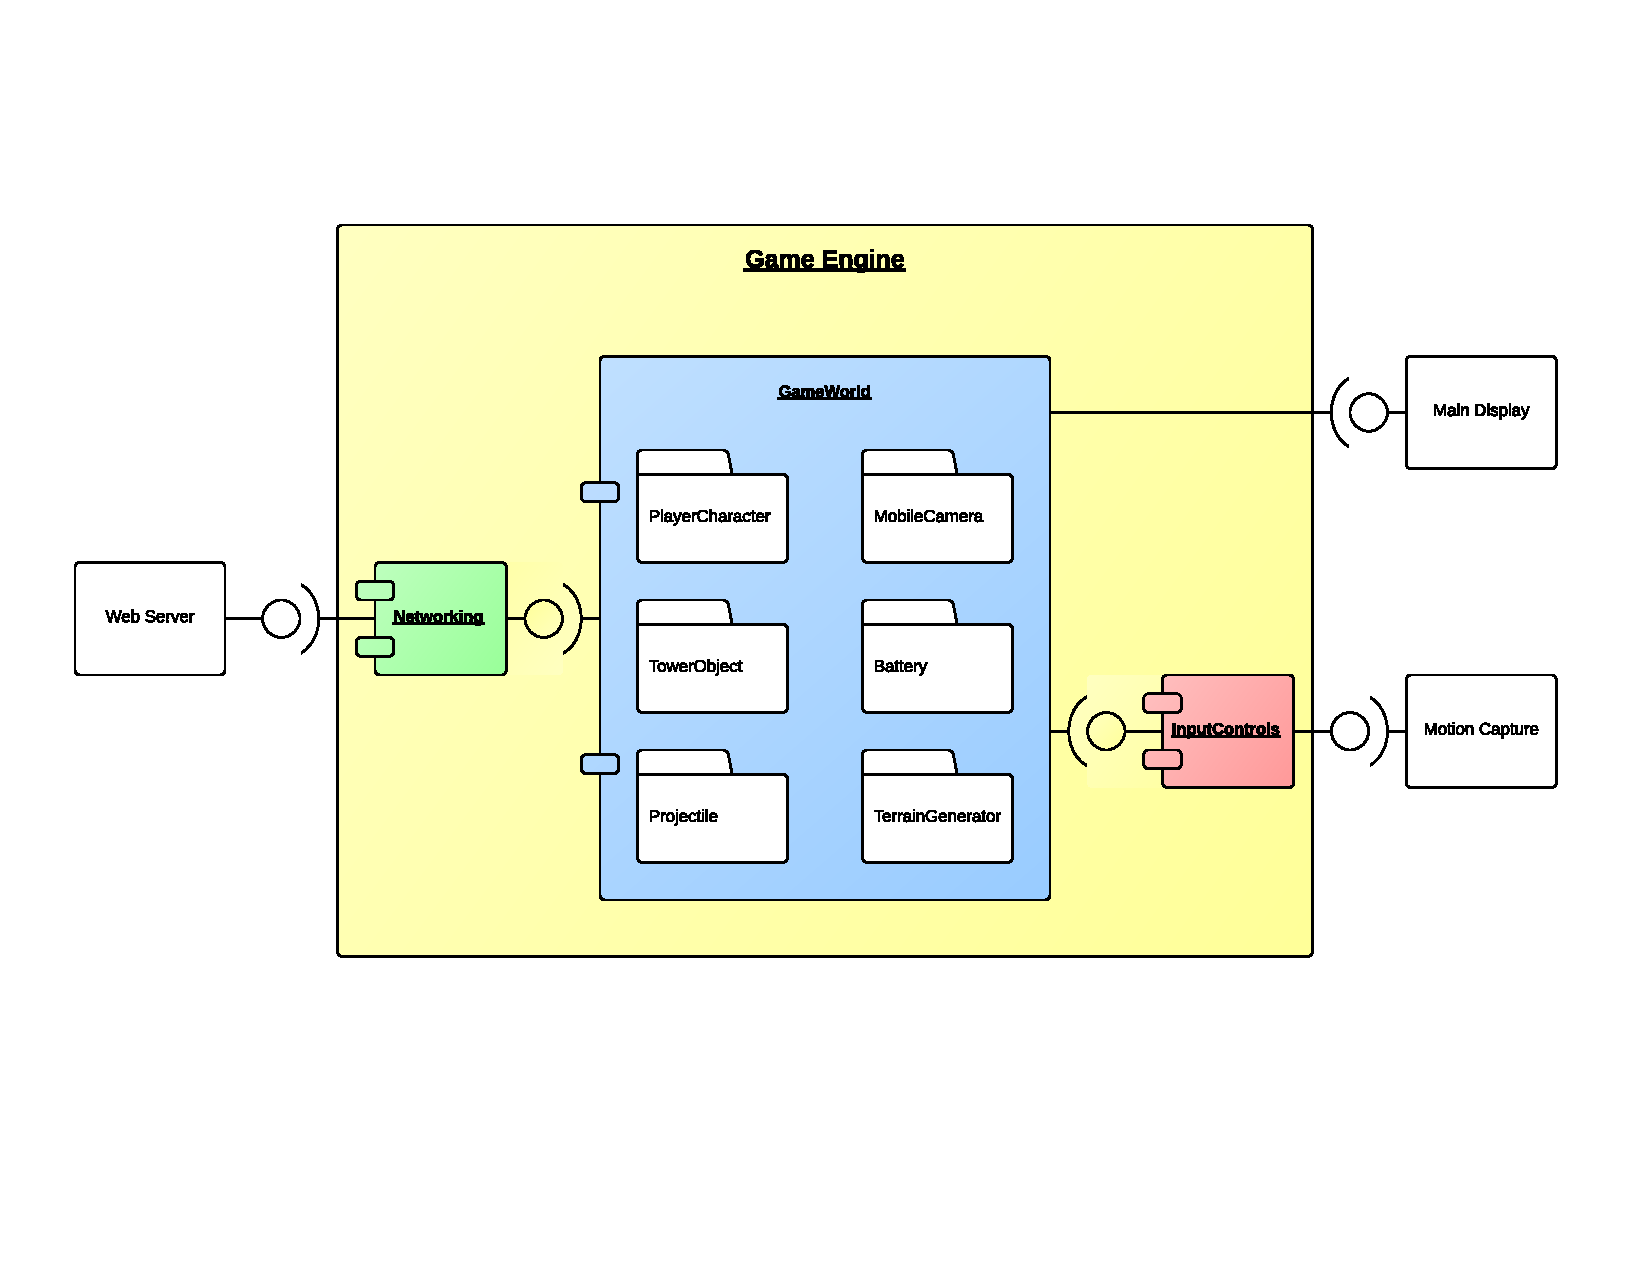
\includegraphics[scale= 0.7]{ComponentDiagram}

\subsection{Algorithms, Design Patterns and Data Structures}
The Class diagram is admittedly complex, so let’s break it down into the most important components. The Networking module has but 2 classes. The NetworkInterface class uses the JSONObject class to exchange JSON objects with the web server. Currently, only one class actually is translated to and from a JSONObject, which is the TowerObject. We have plans to translate the PlayerCharacter into a JSONObject in the very near future.

The InputControls module is even simpler. It has one class which contains variables that are updated by the motion capture group. Every frame, the PlayerCharacter class polls the variables and moves the character accordingly.

The GameWorld module is by far the most complex. At the heart of the module is the PlayerCharacter class, which by necessity interacts with most other classes in the module. There are a number of other classes, for example the TowerObject class, which do something in the game to interact with the character. The TowerObject with shoot bullets at the character if it is within a certain range.

The GameWorld module is separated into a number of sub-modules. Each sub-module is essentially a mental delineation of types of objects in the game. The HUD sub-module contains all of the game data which appears on the heads-up display, such as the energy bar and the player’s score. It retrieves data from the PlayerCharacter about the energy level, and from Items which will be discussed shortly.

The Terrain sub-module is the mechanism for creating the terrain that the character moves on. The terrain in-game consists of a number of TileStates -- giant squares on the ground which can fall away after a period of time. The TerrainGenerator class creates the terrain using a number of these TileStates.

The Item sub-module represents the collection of objects with which the PlayerCharacter interacts. These include powerups and projectiles. The AutoDestroyable superclass provides a mechanism for automatically removing an object from the game after a certain period of time. The RandomObjectFactory sits outside of the Item sub-module but interacts closely with it. Provided a game object, this class will produce clones of that objects throughout the game scene. This is useful, for example, in spawning powerups (like batteries) randomly throughout the game world.

An important note to make is that all of the classes in the GameWorld module inherit from MonoBehavior, which is a class provided by the Unity3D game engine with hooks for performing tasks in a structured order. In particular, it provides two important functions: void Start(), which is called to initialize an object, and void Update(), which is called every frame. These two functions are what allow fluid movement in-game, yet absolute control for the programmer. Additionally, MonoBehavior inherits from GameObject, another Unity-provided class which encapsulates additional information such as mesh rendering, positions, and so forth. The net result is that the classes in the GameWorld module contain this additional information about positioning and other data, but without having to program it ourselves. All of the classes in the GameWorld module implement the two functions Start() and Update(), but to save space, these functions were not included in the class diagram.

We created a few sub-modules in order to mentally separate the tasks within the game world. It makes more sense, for example, to think of Powerups and Fireballs both as items, which behave quite similarly in most circumstances, than as two completely different entities. It simply is a grouping of objects with similar functionalities.

\section{Fault Tolerance}
There is fault tolerance in two places: in the interface to the web server, and in the interface to motion capture. Fault tolerance is not necessary in any other circumstances because the Unity3D engine manages everything related to the game itself; we must only directly ensure that external connections are reliable.

As for the interface to the web server, we use a robust parser to ensure that the data we receive is valid. If any of the data we receive cannot be parsed properly, the data is discarded. At the same time, we will be sending data to the web server as well, and we receive notifications when the data transmissions fail so we can act accordingly. (Note that all transmissions are stateless -- each transmission is independent from the next, so ensuring constant connectivity is not necessary). Thus, there is fault tolerance both when sending and when receiving data.

The interface with motion capture is much simpler. Unlike the web server interface, we simply must ensure that the connection remains active. If it disconnects, we will attempt to reconnect, and possibly pause the game if we are unable to do so (as a user notification).

\section{Local Data Storing}
Currently, we only plan on storing key bindings and other options. Fortunately, all of this is managed by the Unity3D game engine, so we simply have to prompt Unity for everything we need. We have no plans for storing other persistent data ourselves; all persistent storage will be done via the web server (for example, a high score list). It is possible that, in the future, we may save local high score lists and web server information.

\section{Procedures Followed}
\subsection{Development Responsibility}
For the most part, coding has been done on what was interesting to each individual. Below are the general areas of focus. In addition to these, we all shared the responsibility of writing the documentation documents, such as this one, and communication with each other as to what was necessary for the next demonstration session.
\subsubsection{Robin}
\textbf{Animation and Graphics} \\ In general, Robin has worked on the graphics and animation necessary for the game, so far including the Character and Mobile Users.

\subsubsection{Etan}
\textbf{Gameworld Tiles, Usability of Interface} \\ Etan worked mainly on generating and modifying the state of the in-game tile system, as well as work on the Main Menu interface functionality.

\subsubsection{Nick}
\textbf{Turrets and Artificial Intelligence} \\ The actions of the turret being able to track the player’s location and shoot the Character fell under Nick’s umbrella.

\subsubsection{Dan}
\textbf{Network Integration, Character Movement} \\ The reading of information sent from the Web Group was Dan’s area of expertise. In addition to this, he also made the character movement possible.

\subsubsection{Chris}
\textbf{Main Menu Rotation, Gameworld Items} \\ Chris helped provide the Main Menu with the ability to rotate between the various menus, as well as created different items for the gameworld.

\section{Tools Utilized}
We are using the Unity3D game engine for development, Blender for model creation and animations, and Git for source code management (with a main repository stored on GitHub.com). The general process is to always pull down changes before making updates, then modifying files, and submitting those files back to the main repository. The Unity .scene files cannot be merged, so the copies of the .scene files are overwritten with the latest commit.

\section{Testing and Verification Procedures}
Since each individual person had his or her own task, each of us would work on one part of the project, ensure it would work with the character object and then integrate. We would then meet and integrate each of our sections together to test and make sure each individual part is working well together.

We do not have a formal testing process yet, because of the large volume of work that we are completing. However, each member of the group only submits code that at least builds, and we all see each other’s code, so by having multiple viewpoints, we should be able to catch some bugs. As more of the project gets completed, we will have more time to spend validating our code.

Verification of our code is an ongoing process because the nature of the game itself is constantly evolving. In fact, much of game has developed out of what the programmers have created thus far. We essentially are deciding what the game is to become. In this regard, we implicity are verifying the end user’s experience -- we are defining what the user’s experience should be in the first place! 

\section{Coding Conventions}
We are using the programming language C\# in Unity3D. Our choice for this is simply because C\# is one of three languages available to us in this engine (the other two are a derivative of Python called Boo, and a variant of Javascript colloquially called UnityScript), and of the three C\# is both the fastest to learn (with its close parallels to Java) and the fastest at runtime.

In regards to coding conventions, we try to name the variables with very practical names so we can keep track of which variable controls which part of the game. This is necessary because we can serialize variables to view them in the game engine editor (which is useful for changing values in the code without ever having to look at it). Confusing variables would be a nuisance not only to the programmer, but also to the graphic designer who may choose to edit the values of those variables in the Unity game editor. We are also trying to maintain various Unity standards of coding, such as using built-in functions like Start() and Update() and keeping the various inheritance structures that Unity creates for us. In order to have clear, maintainable, and efficient code, we must adhere to these standards of coding.

In regards to comments and coding conventions, because each individual person has been working on different jobs, the conventions for coding and comments vary. For example in the TileDespawner class, there are very few comments. In contrast the PlayerCharacter class has comments sprinkled throughout the code. The Game Design Group’s ideal code has many comments: before each method and inside the method to describe complex algorithms. The code will have very easily identifiable variable names that correspond with the conventions of each class. Likewise the coding conventions with similar indents and spaces between the methods will be the same throughout each class. We should aspire to this level of commenting so that any member of our group (or any other programmer, for that matter) can view the code any other member wrote and easily be able to add or modify code. Comments, quite simply, help to maintain and improve code.

\section{Reflection}
The largest challenge that our group faced was strictly with scheduling. Due to our differing schedules it was challenging to find time, outside of the class-dedicated time, in which we could all meet in order to work together. The difference in our individual schedules and overall lack of set meeting times took its toll on both our documents and coding. We overcame this by having meetings over Google Docs. This allowed us to share our work without everyone having to be at the same place at the same time and also gave us a central place in which we could share thoughts and ideas. This scheduling conflict also caused us to underestimate the time it would take to learn both Unity and Blender.
\subsection{Schedule}
\subsubsection{September}
\begin{description}
	\item [14 Requirements Spec. Due] \textit{complete}
	\item [21 Upload basic Unity3D project to root repository] Writing the design documentation begins. \textit{complete}
\end{description}

\subsubsection{October}
\begin{description}
	\item [2 Design Doc. Due] \textit{complete}
	\item [3 Begin Implementation of Back-end] Back-end functional. \textit{complete}
	\item [8 Integration of Design Docs. with other groups] \textit{complete}
	\item [12 Back-end Complete] \textit{complete}
	\item [19 Essential gameplay Complete, Essential Graphics Complete] Be able to play the game with a keyboard. \textit{complete} Intergration with Kinect begins. \prog
	\item [25 Integration with Kinect complete] Ability to play game via puppeteering and the Kinect. \ncomp
	\item [26 Begin Integration with Android and Augmented Reality Groups] Begin designing a network protocol for the Web group.
\end{description}

\subsubsection{November}
\begin{description}
	\item [2 Network Protocol Design] Network protocol is agreed upon and implementation begins. Implementation of the high score system begins.
	\item [5 Title Screen] Main Menu interface is completely functional with Kinect inputs, and allows the game to be played. \textit{complete}
	\item [16 Network, Android and Augmented Reality Groups Integration] Integration with all other groups is possible. Test document is due.
	\item [21 Networked High Score System Complete] Ability to send and receive high scores from the Web Group will be complete.
	\item [26 Integration] Integration with all other groups fully complete.
	\item [28 ``Bells and whistles'' of gameplay complete] The game is finished in its entirety, and exhaustive testing and bug fixing begins. This will be done by all group members.
\end{description}

\subsubsection{December}
\begin{description}
	\item[10 Vi-Char Complete!] Final Demonstration \& Final Report will be given.
\end{description}

\subsection{Note} We have completed all of the tasks to schedule, except for those related to graphic design. However, we have begun integrating with the web server ahead of schedule. Hopefully, this will offset the slow progress of the graphic design. We fully expect to be on schedule for testing in late November.

\begin{description}
	\item[Communication] Lack of set times to meet took a toll on our work together, especially on the documents and coding, outside of the class-dedicated meeting times.
	\item[3D Modeling] Our group underestimated the amount of time spent to learn Blender.
\end{description}

\section{Glossary and References}

\gls{Avatar}{See Character}

\gls{Blender}{An opensource 3D modeling program}

\gls{Character}{The game object controlled by persons using the Kinect}

\gls{Floating Creatures}{The avatars inside the GameWorld the Mobile Device group control}

\gls{Gamepad}{A human input device with buttons and analog sticks}

\gls{git}{A distributed version control system, which tracks and annotates changes to }code

\gls{Github}{A hosting service for the source code of software projects}

\gls{Google Docs}{A service provided by Google to collaboratively create documents}

\gls{JSON}{JavaScript Object Notation, a text based, human readable, standard for data interchange. \wref}

\gls{Kinect}{A motion capture system, gathers 3D information of puppeteer's locations}

\gls{LaTeX}{A document markup language and preparation system}

\gls{MainDisplay}{The projector that spectators as well as puppeteers will be able to see. Will display the current state of the gameworld.}

\gls{Unity3D}{Integrated authoring tool for creating 3D video games or other interactive content such as architectural visualizations or real-time 3D animations}

\gls{Viewport}{The view seen of the game, similar to an aerial view}


\end{document}
